% Instructions for the researcher documenting how to use the
% AndWellness researcher dashboard.

\documentclass{article}
\usepackage{fullpage}
\usepackage{graphicx}

\title{AndWellness Researcher Dashboard Instructions}

\begin{document}
\maketitle

The main andwellness.org webpage has a basic description of AndWellness and a small
login form in the top right corner.  Enter your user name
and password and click send to enter the main dashboard.  The initial loading of the dashboard may take a few seconds.
If the logged in user is idle for more than 30 minutes, they will be automatically logged out and will have to relogin.

The dashboard layout is separated into the header and the main body.
The header includes the title of the campaign (ABC Study), the
name of the currently logged in user, and two tab buttons to switch among the
dashboard views labeled \emph{Upload Stats} and \emph{EMA Graphs}.

\section*{Upload Statistics}
% Include example image here 
\begin{center}
	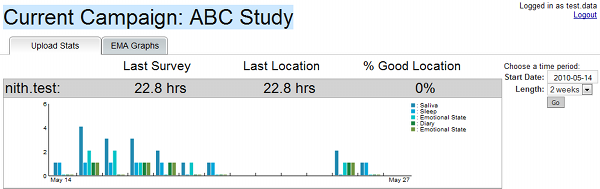
\includegraphics[width=6in]{dashboard-shrunk}
\end{center}

The upload statics view displays all users enrolled in the current
campaign.  Each user has three columns labeled \emph{Last Survey},
\emph{Last Location}, and \emph{\% Good Location}.  The last survey column
displays the time since the last survey was taken in hours and
will show No Data if the user has not yet uploaded data.  The time displayed
is the time since the user took the survey, not the time since the data were uploaded to the server.
The next column, Last Location, displays the time since a good GPS value was received.  A large
value here indicates the user is in a location that has poor GPS reception.  The third column, \% Good Location,
shows the percentage of recent survey uploads that have good GPS data.  Again, a low percentage indicates
poor GPS reception.  This value only takes into account the past 24 hours, if no data has been uploaded in that
time the number will always be 0.

Each user also has a graph to display the number of prompts completed per day in the given time period.
The prompts are counted in five groups: Saliva, Sleep, Emotional State, Diary, and end of day Emotional State.
A full day of prompts should return 4 saliva surveys, 1 sleep survey, 2 emotional state surveys, 1 diary survey, and 
one end of day emotional state survey.  The time period is selected using the controls on the right.  Choose a new starting date
and length of time and click Go to update the graphs.  If there is no data for a user for a selected time period, no graph will show for that user.

\section*{EMA Graphs}
\begin{center}
	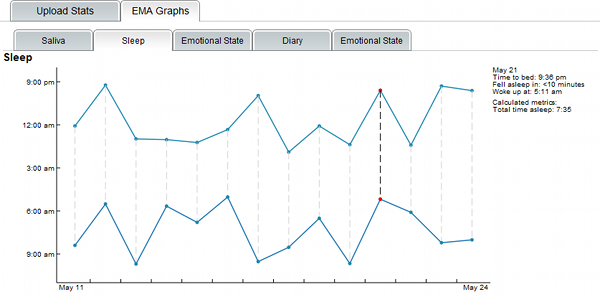
\includegraphics[width=6in]{ema-shrunk}
\end{center}

Click on EMA Graphs to switch to EMA graphing view.  The data is again separated into the same 5 groups: Saliva,
Sleep, Emotional State, Diary, and end of day Emotional State.  Click on any of the 5 sub-tabs to switch among these.
As of now, only data for the current user is shown.  To visualize another users' data, login as that user.

Use the same controls on the right to choose the time period to display.  Click Go to download and visualize
the new time period.  Depending on the speed of your computer and the current load on the server, this may
take a few seconds.   Each of the tabs has a different display:

{\bf Saliva:} Displays a dot for every time a user entered saliva information.  Hover the mouse over the dot
	to check if the user brushed, ate, or drank before taking the saliva sample.

{\bf Sleep:} Displays the daily sleep patterns of the participant from the \emph{Waking} survey.  The top line denotes when the participant
	went to sleep,the bottom line denotes when the participant woke up.  Hover the mouse to see further information
	to the right.

{\bf Emotional State:} Displays information from the \emph{Mid-morning} and \emph{Afternoon} surveys.  Each response
	is shown as a blue bar, and the average response over the time period is displayed on the right.

{\bf Diary:} Displays information from the \emph{Bedtime} survey.

{\bf End of day Emotional State:} Displays information from the \emph{Bedtime} survey.  These prompts ask the participant
	how they felt throughout the day, versus the previous emotional state surveys that ask for the current state of the participant.

\end{document}
